
\subsection{Bayes' Theorem} 

\ssn{Introduction} 
Bayes' Theorem (or sometimes Bayes' ``rule'' or ``formula'') has a simple proof but is of huge importance in  answering questions about how probable it is that some event has ``caused'' an observed result.  It is hugely important in Statistics: there is a whole approach to statistical analysis using ``Bayesian methods''.  It is fundamental also in machine learning. 
\end{n}

\ssn{Conditional probability revisited}
I toss a coin 5 times and obtain 3 or more heads.  What is the probability that the first toss was H? 

Let $B$ be the event of 3 or more H out of 5.  Then by binomial 
 \[
     \PP( B) = \frac1{2^5}\left(  \binom53 + \binom54 + \binom55 \right)   =  \frac{16}{2^5}.
 \]
Let $A$ be the event that the first toss is H.  Then $A \cap B$ is the event of tossing a H, followed by at least 2 H in the remaining 4 tosses. So by binomial again 
 \[
   \PP(A \cap B) = \frac12 \; \frac1{2^4} \left(  \binom42 + \binom43 +\binom 44\right) = \frac{11}{2^5}.
 \]
 So dividing, 
  \[
  \PP(A \st B) = \frac{11/2^5}{16/2^5} = \frac{11}{16}.  
 \]

\end{n}

\ssn{``Zooming in''}
In taking probabilities conditional upon an event $B$, one is zooming in on $B$, replacing ones initial sample space $S$ with $B$. In doing so, one becomes interested in $A \cap B$ rather than $A$ itself.  Figure~\ref{condo} illustrates what is going on. 
\end{n}


\begin{figure}[h] \centering
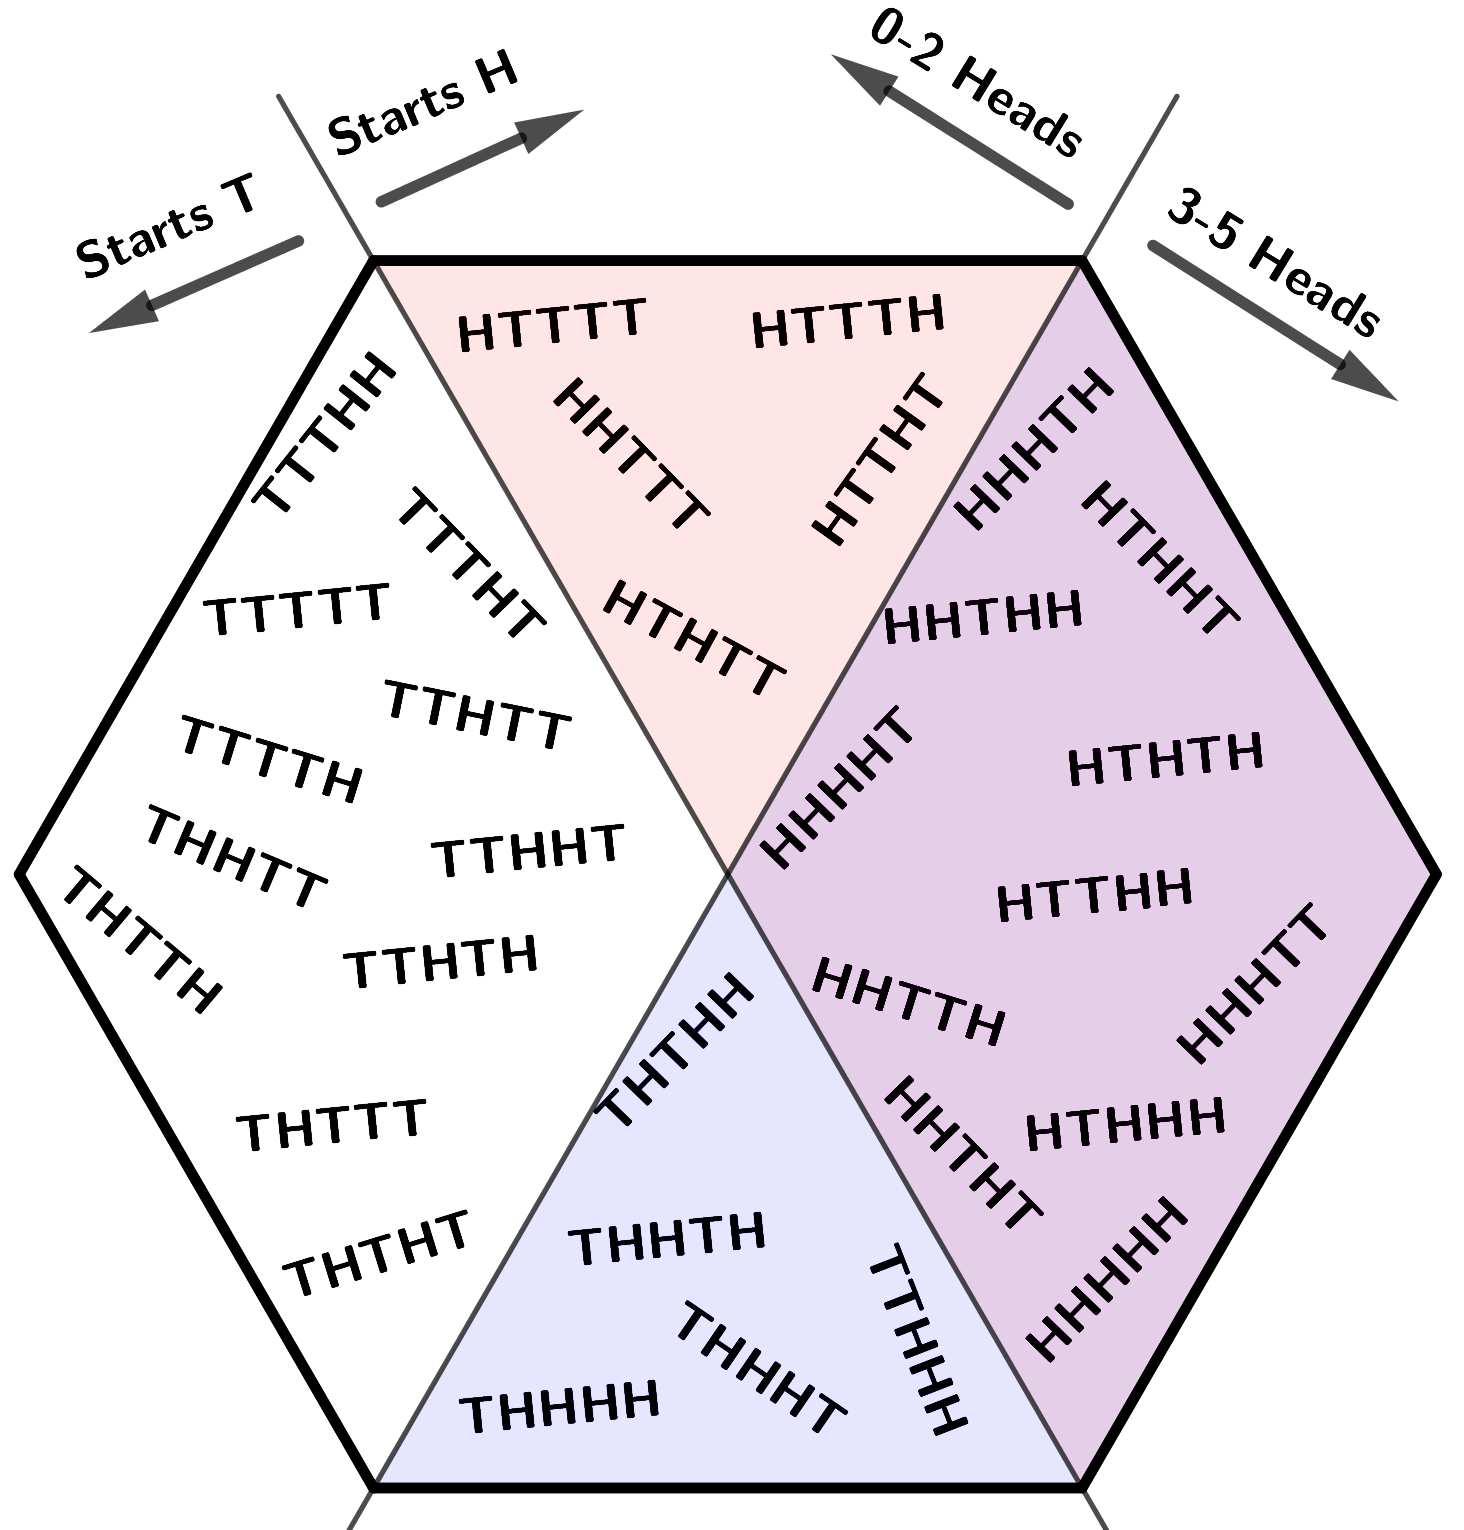
\includegraphics[width=0.52\textwidth]{images/condo0.png}\qquad
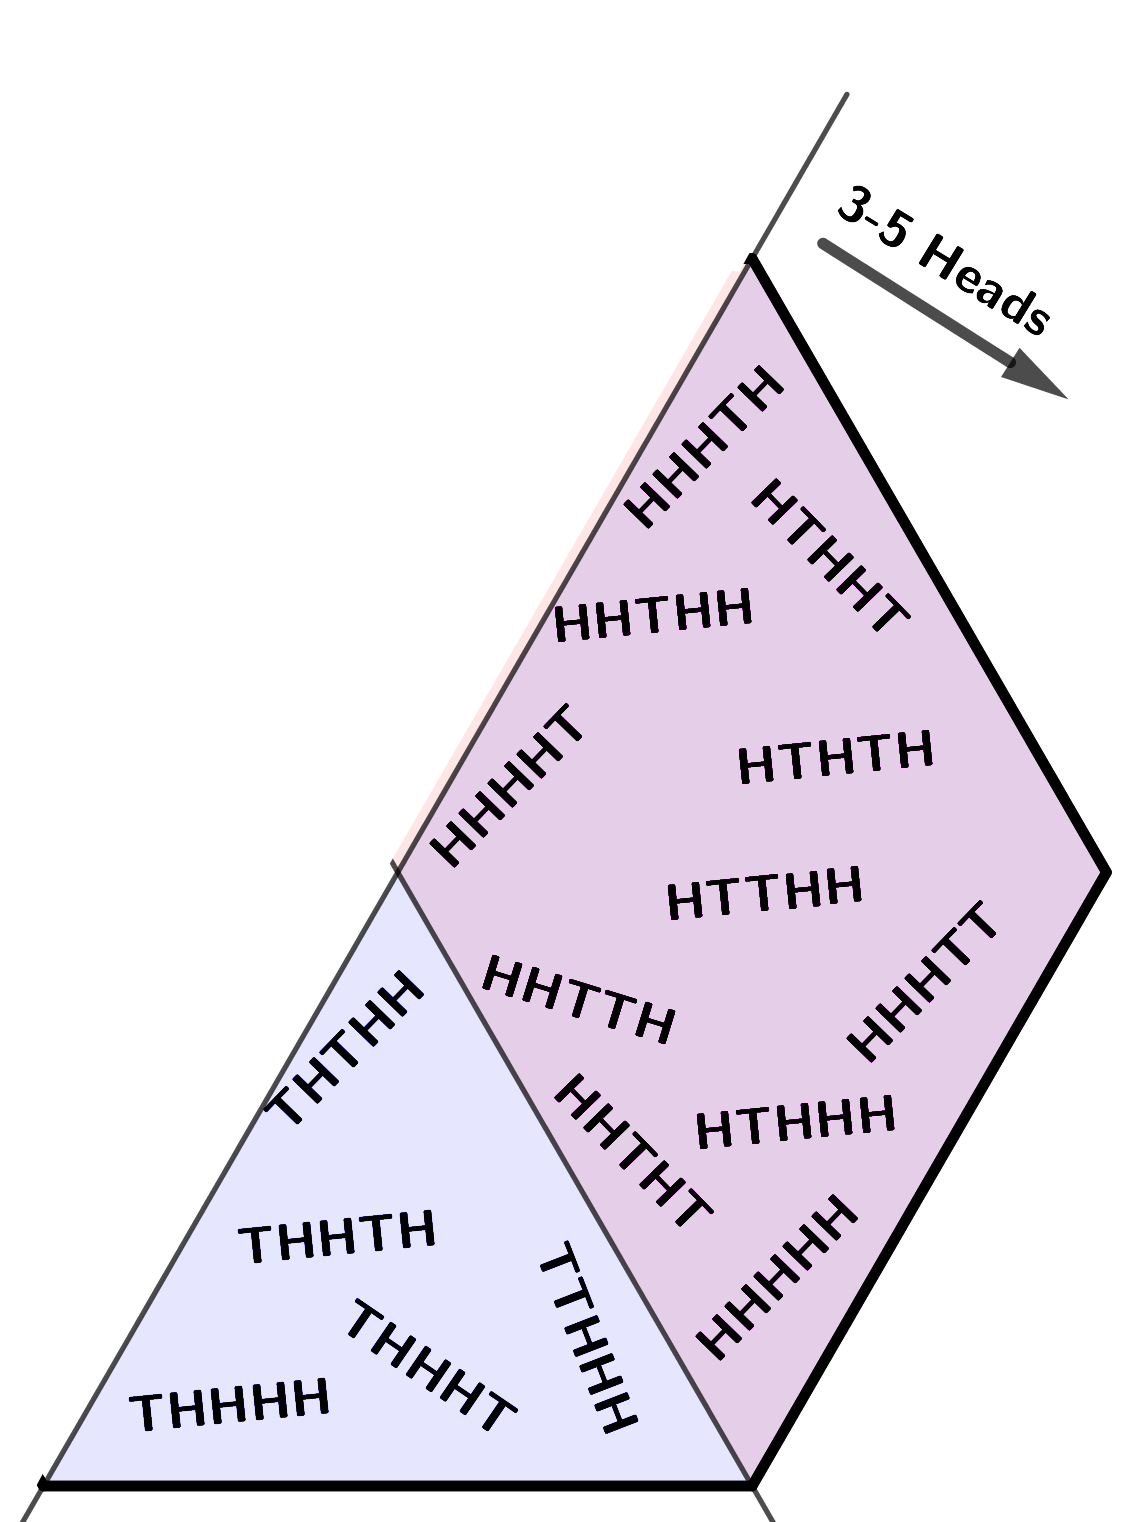
\includegraphics[width=0.4\textwidth]{images/condo1.png}
\caption{\label{condo} The whole sample space for 5 coin tosses (left). ``Zooming in'' on the half with $\geq 3$ heads, we see that $11/16$ start with an `H'. So $\PP(\text{starts with H} \st \text{number of H $\geq 3$ }) = 11/16$.} 
\end{figure}

\ssn{Bayes' Theorem} 
Let $A,B$ be events with $\PP(B)\not= 0$.  Then 
\tcb  
\[
    \PP( A \st B) = \PP( B \st A) \frac{\PP(A)}{\PP(B)}.
 \]
\etcb 
\begin{proof}
We compute $\PP(A \cap B)$ in two different ways: 
 \[ 
 \PP(B \st A) \PP(A) = \PP(A \cap B) = \PP(A \st B) \PP(B). 
 \]
Dividing by $B$ gives the result. 
\end{proof}
We could easily have solved the problem above using Bayes' Theorem; it would be essentially the same calculation. 
\end{n}

\ssn{Bayes' Theorem (``probability of causes'' form) }
Let our sample space $S$ be partitioned into disjoint events $A_k, \, k=1,2,\dots, n$.  Then for $1\leq j \leq n$, 
\tcb
\[
   \PP(A_j \st B)  =   \frac{\PP(B \st A_j)\,\PP(A_j)}{ \sum_{k=1}^n \PP(B \st A_k) \,\PP(A_k)}
 \]
 \etcb 
\begin{proof}
Put $A=A_j$ in the previous version of the theorem and then expand $\PP(B)$ using the law of total probability (\S\ref{totprob}).
\end{proof}
\end{n}

\ssn{Example}
The use of the the ``probability of causes'' form is more straightforward than it might appear from the statement. 

Tom and Dick are both liars: independently for everything they say, they tell the truth with probability $1/3$ and lie with probability $2/3$.  Tom says something.  Dick tells me that Tom is telling the truth.  What is the probability that Tom is telling the truth? 


\tikzset{
  treenode/.style = {shape=rectangle, rounded corners,
                     draw, align=center,
                     top color=white, bottom color=blue!30},
  root/.style     = {treenode, font=\Large, bottom color=red!30},
  env/.style      = {treenode},
  branch/.style = {treenode, bottom color=blue!10},  
  dummy/.style    = {circle,draw}
}
\tikzstyle{level 1}=[level distance=4.0cm, sibling distance=3.5cm]
\tikzstyle{level 2}=[level distance=5.0cm, sibling distance=2.0cm]

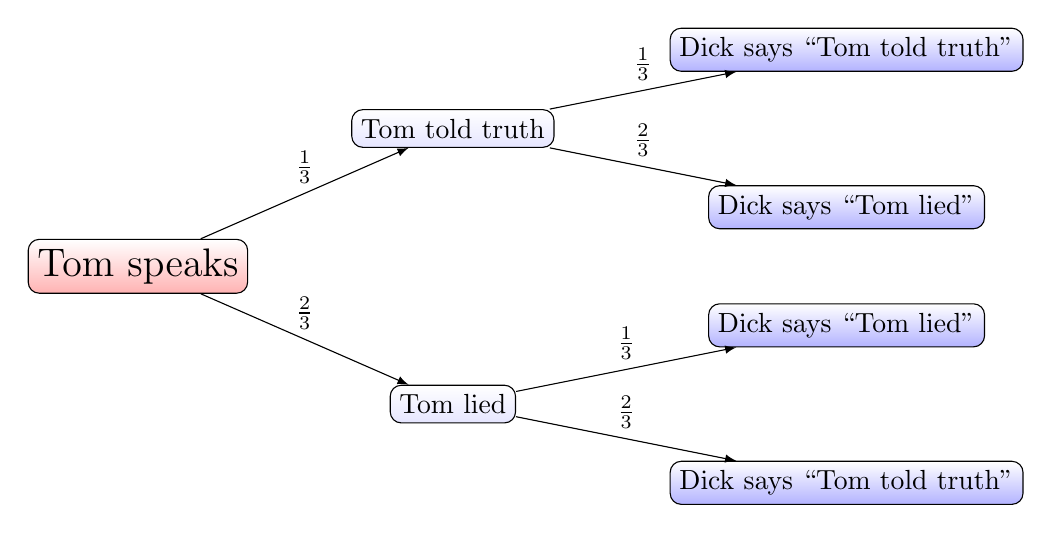
\begin{tikzpicture}
[
grow=right,
    edge from parent/.style = {draw, -latex},
    every node/.style       = {font=\normalsize}
  ]
\node[root]{Tom speaks}
child { 
    node[branch]{Tom lied}
    child { 
        node[env]{Dick says ``Tom told truth''}  
        edge from parent node[above]{$\frac23$} 
        }       
    child { 
        node[env]{Dick says ``Tom lied''}                 
        edge from parent node[above]{$\frac{1}{3}$} 
        }       
    edge from parent node[above]{$\frac23$}            
    }
child { 
    node[branch]{Tom told truth}
    child { 
        node[env]{Dick says ``Tom lied''}                
        edge from parent node[above]{$\frac{2}{3}$} 
        }       
    child { 
        node[env]{Dick says ``Tom told truth''}               
        edge from parent node[above]{$\frac{1}{3}$} 
        }       
    edge from parent node[above]{$\frac{1}{3}$}            
    }     ;           
\end{tikzpicture}

Here, we let $A_1$ be ``Tom told truth'' and let $A_2$ be ``Tom lied''.    We let $B$ be the event that ``Dick says Tom told truth''. 
We are asked to calculate $\PP( A_1 \st B)$. So, using Bayes' theorem in the ``probability of causes'' version we have 
 \begin{eqnarray*}
   \PP( A_1 \st B) &=& 
     \frac{\PP(B \st A_1) \, \PP(A_1)}
     {  \PP(B \st A_1) \,\PP(A_1) + \PP(B \st A_2)\,
         \PP(A_2)   } \\
    &=& \frac{ (1/3)(1/3)}{(1/3)(1/3)+(2/3)(2/3)}  = \frac15. 
 \end{eqnarray*}
\end{n}

\ssn{Example}
The example we will now study is presented as an ``updating information'' example where we use the original Bayes' theorem.  You might like to convert it to a ``probability of causes'' wording and draw the probability tree to understand the connection.

A suspect X is believed to be guilty of a given crime with probability $\PP(G)=0.6$ on the basis of existing evidence.  The criminal also left a blood stain at the scene. The suspect X has a blood group common to 20\% of the general population.

A test on the blood stain now tells us that it comes from a person with this blood group. How does that affect the probability that the suspect X is guilty? 


Let $B$ be the event that the blood stain has this particular blood group.  We know the blood test will certainly be positive if X is guilty, so $\PP( B \st G) = 1$.  But we want to know the probability of X's guilt, given the new evidence. In other words, we want to find $\PP( G \st B)$. 


First we calculate (law of total probability again) 
 \begin{eqnarray*}
  \PP(B) &=& \PP(\text{X guilty}) \,\PP(B \st \text{X guilty})   + \PP(\text{X not guilty}) \,  \PP(B \st \text{X not guilty} ) \\
  &=& (0.6) (1) + (0.4) (0.2)  = 0.68
 \end{eqnarray*}
 because if X is not guilty, the blood test will be positive with the probability of its being so in the general population.
 
Then according to Bayes' Theorem
 \[
    \PP( G \st B) =  \frac{\PP( B \st G)}{\PP(B)} \, \PP(G)
    =  \frac{1}{0.68} \, 0.6 = 0.88 
 \]
is an updated probability of X's guilt. 

Bayes' Theorem has been widely used in court cases. See \url{https://www.theguardian.com/law/2011/oct/02/formula-justice-bayes-theorem-miscarriage} for a controversy a few years ago around this. (Colin Aitken, until recently in the School of Mathematics in Edinburgh is quoted.) 
\end{n}

\sse{}
I toss a coin 6 times and get a total of four heads. What is the probability my first roll was heads?  (Ans: $2/3$.) 
\end{e}



\subsection{Exercises} 


\sse 
A very standard example of this sort of ``probability of causes'' analysis is ``false positives'' in medicine. For example, suppose that in the general population, a certain condition is present in 1\% of people.  

There is a test for the condition. The test always returns positive if the subject has the condition.  If the subject does not have the condition, it returns negative 95\% of the time but gives a positive response 5\% of the time.  

A random person takes the test and it returns positive. What is the probability they have the disease? 
\end{e}

\sss 
You may find drawing the tree helps.   In this case, let $C$ denote the event that the random person has the condition.  Let $T$ denote the event of a positive test result.  From the question 
 \[  
    \PP(C) = 0.01, \quad \PP(C^c) = 0.99, \quad \PP(T \st C) = 1, 
    \quad \PP( T \st C^c)=0.05
 \] 
 where the complement $C^c$ is the event of the person not having the condition. Finally, 
 \[
 \PP(T) = \PP(T \st C) \PP(C) + \PP(T \st C^c) \PP(C^c) = 
   1 (0.01) + 0.05 ( 0.99) = 0.0496.
 \]
We are asked for $\PP( C \st T)$ and so by Bayes,
\[
   \PP(C \st T) = \PP(T \st C) \,\frac{\PP(C)}{\PP(T)} 
   = 1 \; \frac{0.01}{0.0496} = 0.2016. 
\]
(One sees here a basic problem with ``screening'' programmes: unless the test is very reliable, they will throw up many more false alarms than real ones.) 
\end{s}



\sse 
This sort of information updating with Bayes' Theorem is also an essential ingredient in machine learning. It goes something like this. 

Suppose an image identifying algorithm is trying to decide what sort of animal is appearing in a picture on the web.  The word ``cat'' appears in nearby text so the algorithm's initial hypothesis is it's a cat with probability $0.8$. The algorithm decides that there is a ball of string in the picture. It is known that this is the case for 50\% of cat pictures but also for 10\% of non-cat pictures.  What is the updated probability that the picture shows a cat? 
\end{e}

\sss
Here $P(C)0.8$, where $C$ is the event of the picture being of a cat. The probability of a ball of string in the picture is 
 \[
   \PP(S) = \PP(S \st C) \PP(C) + \PP(S \st C^c) \PP(C^c) = 
    0.5 * 0.8 + 0.1 * 0.2 = 0.42,  
 \]
(where $C^c$ is the complement of $C$, i.e.\ the even of the picture not being of a cat).   So, by Bayes: 
 \[
   \PP(C \st S) = \frac{\PP(S \st C)}{\PP(S)} \,\PP(C) =
       \frac{0.5}{0.42} 0.8 = 0.95.
 \]
\end{s}

\ssp 
Tom, Dick and Harry each tell the truth independently with probability $1/3$ and lie with probability $2/3$ every time they speak. Tom says something we don't hear; Dick states whether Tom told the truth or not, but we don't hear that either. Harry says that Dick says that Tom told the truth.  What is the probability that Tom told the truth? 
\end{e}

\sss
From a tree, I compute that Harry says that Dick says that Tom told the truth (``HSDSTTT") with probability $13/27$. Also, the conditional probability that Harry says this given that Tom told the truth (``TTT'') is $5/9$. From Bayes (or just analysing the tree),
 \[
   \PP(TTT \st HSDSTTT ) = \PP( HSDSTTT \st TTT) \frac{\PP(TTT)}{\PP(HSDSTTT)} = \frac59 \, \frac{1/3}{13/27} = \frac5{13}. 
 \]
\end{s}


